\documentclass[12pt, a4paper]{report}

 
\usepackage[extrafootnotefeatures]{xepersian}
\usepackage{amsmath}
\usepackage{graphicx}
\usepackage[colorlinks=true, linkcolor=black, urlcolor=darkgray, citecolor=black]{hyperref}
\usepackage{listings}
\usepackage{xcolor} 
\usepackage{afterpage}
\usepackage{setspace}
\usepackage[backend=biber, style=numeric, sorting=none]{biblatex}
\addbibresource{references.bib}


\onehalfspacing

\definecolor{codegreen}{rgb}{0,0.6,0}
\definecolor{codegray}{rgb}{0.5,0.5,0.5}
\definecolor{codepurple}{rgb}{0.58,0,0.82}
\definecolor{backcolour}{rgb}{0.95,0.95,0.92}

\lstdefinestyle{mystyle}{
	backgroundcolor=\color{backcolour},   
	commentstyle=\color{codegreen},
	keywordstyle=\color{magenta},
	numberstyle=\tiny\color{codegray},
	stringstyle=\color{codepurple},
	basicstyle=\ttfamily\footnotesize,
	breakatwhitespace=false,         
	breaklines=true,
	captionpos=b,
	keepspaces=true,
	numbers=left,
	numbersep=5pt,
	showspaces=false,
	showstringspaces=false,
	showtabs=false,                  
	tabsize=2,
	language=Python
}

\lstset{style=mystyle}
\renewcommand{\labelitemi}{-}

\settextfont{XB Niloofar}

\newcommand\blankpage{%
	\null
	\thispagestyle{empty}%
	\addtocounter{page}{-1}%
	\newpage}
	
	
\begin{document}
	\blankpage

	\begin{center}
		
\includegraphics{besm1.jpg}
	\end{center}
	\thispagestyle{empty}
	\begin{center}
		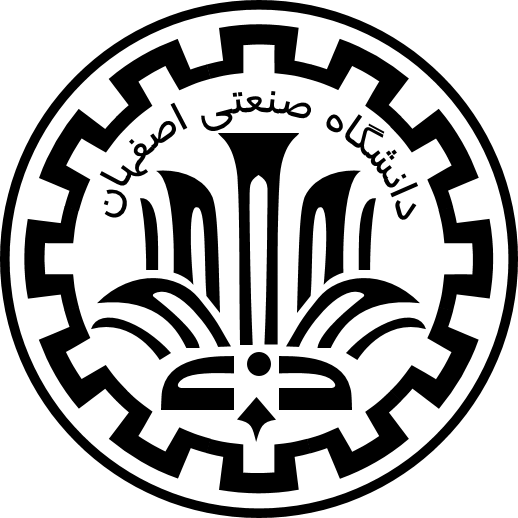
\includegraphics[height=3cm]{iut_logo.png}
		\vspace{0.4cm}
		
		\textbf{دانشگاه صنعتی اصفهان}\\
		\vspace{0.4cm}
		
		{\large
			
			دانشکده مهندسی برق و کامپیوتر
		}
		\vspace{2cm}
		
		{\Large
			\textbf{بررسی و تحلیل حریم خصوصی در شبکه بلاکچین}\\
		}
		\vspace{3cm}
		
		{\Large
			پایان‌نامه کارشناسی مهندسی کامپیوتر - نرم افزار\\
		}
		\vspace{1cm}
		
		{\large
			\textbf{امیرحسین لوافی}\\
		}
		\vspace{3cm}
		
		{\large

		}
		\vspace{0.5cm}
		
		{\large
			\textbf{دکتر مجتبی خلیلی}\\
		}
		\vspace{1cm}
		
		\textbf{1404}
		
	\end{center}

	\pagebreak




	\tableofcontents
	\newpage
	
	\chapter{مقدمه}
\label{chap:introduction}

بلاکچین، فناوری زیربنایی ارزهای دیجیتالی مانند بیت‌کوین، اغلب با کلیدواژه‌هایی مانند «شفافیت»، «تغییرناپذیری» و «ناشناسی»\LTRfootnote{Anonymous} توصیف می‌شود. در حالی که دو ویژگی اول تا حد زیادی صحیح هستند، ویژگی سوم، یعنی ناشناسی، یکی از بزرگ‌ترین و رایج‌ترین تصورات غلط در مورد این فناوری است. در حقیقت، اکثر بلاکچین‌های عمومی مانند بیت‌کوین، ناشناس نیستند، بلکه «شبه‌ناشناس»\LTRfootnote{Pseudonymous} هستند \cite{antonopoulos_mastering}. این تمایز ظریف، نقطه آغازین بحث پیچیده و حیاتی «حریم خصوصی در بلاکچین» است.

در این گزارش، ما به بررسی عمیق مفهوم حریم خصوصی در بستر بلاکچین، با تمرکز ویژه بر شبکه بیت‌کوین، خواهیم پرداخت. ابتدا به این پرسش پاسخ می‌دهیم که حریم خصوصی در این اکوسیستم دیجیتال به چه معناست، سپس اهمیت آن را در ابعاد مختلف تحلیل کرده و در نهایت، به چالش‌ها و خطراتی می‌پردازیم که نقض حریم خصوصی می‌تواند برای کاربران به همراه داشته باشد.

\section{حریم خصوصی در بلاکچین چیست؟}

بر خلاف سیستم‌های مالی سنتی، در بلاکچین بیت‌کوین تمام تراکنش‌ها در یک «دفتر کل عمومی و توزیع‌شده»\LTRfootnote{Public Ledger} ثبت و برای همگان قابل مشاهده است \cite{nakamoto_whitepaper}. هر کسی می‌تواند مقدار بیت‌کوین منتقل‌شده، آدرس‌های فرستنده و گیرنده، و زمان دقیق هر تراکنش را از ابتدای پیدایش شبکه تا به امروز مشاهده کند.

در این سیستم، هویت کاربران پشت آدرس‌های رمزنگاری‌شده پنهان می‌شود. این آدرس‌ها رشته‌هایی طولانی از حروف و اعداد هستند (مانند \lr{\texttt{1A1zP1eP5QGefi2DMPTfTL5SLmv7DivfNa}}) که هیچ اطلاعات هویتی مستقیمی از صاحب خود را فاش نمی‌کنند. این همان «شبه‌ناشناسی» است: تراکنش‌های شما عمومی هستند، اما هویت واقعی شما (در حالت ایده‌آل) خصوصی باقی می‌ماند. حریم خصوصی در این بستر، به معنای «توانایی یک کاربر برای انجام تراکنش بدون آنکه دیگران بتوانند آن تراکنش را به هویت واقعی او در دنیای فیزیکی مرتبط کنند» تعریف می‌شود.

\section{چرا حریم خصوصی برای ما مهم است؟}

اهمیت حریم خصوصی در یک سیستم مالی شفاف مانند بلاکچین، فراتر از پنهان کردن فعالیت‌های غیرقانونی است و جنبه‌های حیاتی برای آزادی فردی و کارایی اقتصادی دارد.

\begin{itemize}
	\item \textbf{امنیت شخصی و مالی:} اگر تمام دارایی و تاریخچه تراکنش‌های یک فرد برای عموم قابل مشاهده باشد، آن فرد به یک هدف برای سارقان، هکرها و باج‌گیران تبدیل می‌شود. دانستن اینکه یک آدرس خاص حاوی میلیون‌ها دلار بیت‌کوین است، انگیزه‌ای قوی برای حمله به صاحب آن آدرس ایجاد می‌کند.
	
	\item \textbf{حفظ اطلاعات تجاری:} شرکت‌ها و کسب‌وکارها نمی‌توانند اطلاعات مالی خود، مانند حقوق کارمندان، حجم معاملات با تأمین‌کنندگان، و استراتژی‌های سرمایه‌گذاری را به صورت عمومی فاش کنند. شفافیت کامل، مزیت رقابتی آن‌ها را از بین می‌برد.
	
	\item \textbf{مقاومت در برابر سانسور و کنترل:} در کشورهایی با نظام‌های سیاسی سرکوبگر، حریم خصوصی مالی به مخالفان سیاسی، روزنامه‌نگاران و فعالان حقوق بشر اجازه می‌دهد تا بدون ترس از مسدود شدن حساب‌ها یا ردیابی توسط دولت، به فعالیت‌های خود ادامه دهند.
	
	\item \textbf{تعویض‌پذیری:}\LTRfootnote{Fungibility} این یک مفهوم کلیدی اقتصادی است که می‌گوید هر واحد از یک کالا یا پول باید با واحد دیگری از همان نوع قابل تعویض و دارای ارزش یکسان باشد \cite{antonopoulos_mastering}. اما در بیت‌کوین، اگر تاریخچه یک کوین نشان دهد که در گذشته در یک فعالیت غیرقانونی استفاده شده، ممکن است برخی صرافی‌ها از پذیرش آن خودداری کنند. این «کوین‌های لکه‌دار» ارزش کمتری نسبت به «کوین‌های تمیز» پیدا می‌کنند و خاصیت تعویض‌پذیری بیت‌کوین را تضعیف می‌کنند.
\end{itemize}

\section{خطرات و چالش‌های حریم خصوصی ناکافی}

همانطور که اشاره شد، شبه‌ناشناسی بیت‌کوین یک سپر شکننده است. «شرکت‌های تحلیل بلاکچین»\LTRfootnote{Blockchain Analysis Firms} با استفاده از تکنیک‌های پیشرفته داده‌کاوی، می‌توانند الگوهای رفتاری کاربران را شناسایی کرده و آدرس‌های مختلف را به یک نهاد واحد متصل کنند (فرآیندی به نام «تحلیل خوشه‌ای»\LTRfootnote{Clustering}). این شرکت‌ها با تحلیل گراف تراکنش‌ها و ترکیب آن با «اطلاعات خارج از زنجیره»\LTRfootnote{Off-chain Data}، مانند اطلاعات «احراز هویت»\LTRfootnote{Know Your Customer (KYC)} از صرافی‌ها، می‌توانند هویت واقعی صاحبان آدرس‌ها را با دقت بالایی کشف کنند \cite{narayanan_deanonymizing}.

این فرآیند که «هویت‌زدایی»\LTRfootnote{Deanonymization} نام دارد، خطرات جدی به همراه دارد:
\begin{enumerate}
	\item \textbf{نظارت گسترده:} دولت‌ها و شرکت‌های بزرگ می‌توانند تمام فعالیت‌های مالی افراد را زیر نظر بگیرند. این اطلاعات می‌تواند برای اهداف تبلیغاتی، کنترل اجتماعی یا حتی سرکوب سیاسی مورد استفاده قرار گیرد.
	
	\item \textbf{نقض حریم خصوصی گذشته:} از آنجایی که بلاکچین تغییرناپذیر است، یک اشتباه کوچک در مدیریت حریم خصوصی (مانند استفاده مجدد از یک آدرس) می‌تواند تمام تراکنش‌های گذشته و آینده شما را برای همیشه به هویت‌تان پیوند بزند.
	
	\item \textbf{تبعیض مالی:} اطلاعات مربوط به نحوه خرج کردن پول توسط افراد می‌تواند منجر به تبعیض شود. برای مثال، ممکن است یک شرکت بیمه بر اساس تاریخچه خرید شما، نرخ بالاتری را برایتان تعیین کند یا یک بانک بر اساس الگوی تراکنش‌هایتان، از ارائه وام به شما خودداری کند.
\end{enumerate}

بنابراین، حریم خصوصی در بلاکچین یک مفهوم صفر و یک نیست، بلکه یک طیف است. درک آسیب‌پذیری‌ها و ابزارهای موجود برای تقویت آن، برای هر کاربری که به دنبال حفظ حاکمیت مالی و امنیت خود در این دنیای جدید است، امری ضروری محسوب می‌شود.
	\chapter{تحلیل زنجیره و آسیب‌پذیری‌های حریم خصوصی در بیت‌کوین}
\label{chap:analysis_vulnerabilities}

در فصل مقدمه، به این حقیقت پرداختیم که بیت‌کوین برخلاف تصور عمومی، ناشناس نیست، بلکه «شبه‌ناشناس»\LTRfootnote{Pseudonymous} است. این شبه‌ناشناسی بر این فرض استوار است که ارتباطی بین آدرس‌های روی بلاکچین و هویت‌های واقعی در دنیای خارج وجود ندارد. اما این فرض، یک سپر بسیار شکننده است. در این فصل، به صورت فنی و دقیق بررسی خواهیم کرد که این سپر چگونه شکسته می‌شود. ما به تحلیل ساختار داده‌ای بیت‌کوین می‌پردازیم و تکنیک‌هایی را که توسط شرکت‌های تحلیل بلاکچین برای هویت‌زدایی کاربران به کار می‌رود، تشریح می‌کنیم. درک عمیق این آسیب‌پذیری‌ها، پیش‌نیاز درک اهمیت راهکارهایی است که در فصول بعدی به آن‌ها خواهیم پرداخت.

\section{مدل خروجی خرج‌نشده تراکنش}

برای درک چگونگی ردیابی تراکنش‌ها در بیت‌کوین، ابتدا باید مدل حسابداری آن را بشناسیم. بیت‌کوین از «مدل حساب و موجودی»\LTRfootnote{Account/Balance Model} که در بانکداری سنتی یا بلاکچین‌هایی مانند اتریوم رایج است، استفاده نمی‌کند.

در مقابل، بیت‌کوین بر اساس مدل «خروجی خرج‌نشده تراکنش»\LTRfootnote{Unspent Transaction Output (UTXO)} کار می‌کند \cite{antonopoulos_mastering}. این مدل شباهت زیادی به استفاده از پول نقد فیزیکی دارد. کیف پول شما حاوی یک موجودی کلی نیست، بلکه مجموعه‌ای از اسکناس‌ها و سکه‌های مجزا (همان \lr{UTXO}ها) است. برای درک بهتر، یک مثال را در نظر بگیرید:
فرض کنید شما در کیف پول خود دو \lr{UTXO} مجزا دارید. حال می‌خواهید یک کالایی را بخرید که ارزش آن از هر یک از \lr{UTXO}های شما بیشتر است. شما باید هر دو \lr{UTXO} را به عنوان «ورودی»\LTRfootnote{Input} تراکنش خود «خرج» کنید. تراکنش شما دو «خروجی»\LTRfootnote{Output} جدید ایجاد می‌کند: یکی برای فروشنده و دیگری که به عنوان «باقی‌مانده» به یک آدرس جدید تحت کنترل خودتان برمی‌گردد.

نکته کلیدی این است که هر تراکنش، \lr{UTXO}های قبلی را مصرف کرده و \lr{UTXO}های جدیدی را خلق می‌کند. این فرآیند یک زنجیره‌ی به هم پیوسته از تراکنش‌ها را از گذشته تا به امروز ایجاد می‌کند که کاملاً شفاف و قابل ردیابی است. این شفافیت رادیکال، سنگ بنای تحلیل بلاکچین است.

\section{استفاده مجدد از آدرس: پاشنه آشیل حریم خصوصی}

اگر مدل \lr{UTXO} سنگ بنای تحلیل است، «استفاده مجدد از آدرس»\LTRfootnote{Address Reuse} بزرگ‌ترین اشتباهی است که یک کاربر می‌تواند مرتکب شود \cite{antonopoulos_mastering}. یک آدرس بیت‌کوین از نظر فنی برای یک بار استفاده طراحی شده است. کیف پول‌های مدرن که از «استانداردهای سلسله‌مراتبی قطعی»\LTRfootnote{Hierarchical Deterministic (HD) wallets} پیروی می‌کنند، برای هر تراکنش ورودی یک آدرس کاملاً جدید ایجاد می‌کنند. با این حال، بسیاری از کاربران به دلایل سادگی، یک آدرس ثابت را برای دریافت تمام وجوه خود به دیگران اعلام می‌کنند.

این کار معادل این است که شما تمام درآمدهای خود از منابع مختلف را به یک حساب بانکی شفاف و عمومی واریز کنید. این عمل بلافاصله تمام این نهادها را به یکدیگر و به یک هویت واحد (شما) مرتبط می‌سازد. برای مثال، اگر از یک صرافی معتبر که در آن «احراز هویت»\LTRfootnote{Know Your Customer (KYC)} کرده‌اید، مقداری بیت‌کوین به آدرس \lr{A} خود منتقل کنید و سپس دوست شما نیز به همان آدرس \lr{A} پولی واریز کند، یک تحلیلگر خارجی می‌تواند به راحتی این دو تراکنش را به هویت واقعی شما پیوند بزند.

\section{روش‌های اکتشافی: هنر تبدیل داده به اطلاعات}

شرکت‌های تحلیل بلاکچین صرفاً به داده‌های خام نگاه نمی‌کنند؛ آن‌ها از الگوریتم‌ها و «روش‌های اکتشافی»\LTRfootnote{Heuristics} برای استخراج اطلاعات معنادار از این داده‌ها استفاده می‌کنند \cite{narayanan_deanonymizing}. یک روش اکتشافی، یک قانون سرانگشتی یا یک فرض منطقی است که اگرچه صحت آن ۱۰۰٪ تضمین‌شده نیست، اما در اکثر موارد درست عمل می‌کند.

مهم‌ترین روش اکتشافی در تحلیل بیت‌کوین، «فرض مالکیت مشترک ورودی‌ها»\LTRfootnote{Common-Input-Ownership Heuristic} است. این اصل بیان می‌کند که اگر یک تراکنش چندین ورودی (\lr{UTXO}) داشته باشد، به احتمال بسیار زیاد تمام آن ورودی‌ها توسط یک شخص یا یک کیف پول کنترل می‌شوند. با استفاده مکرر از این روش، تحلیلگران فرآیندی به نام «خوشه‌بندی آدرس»\LTRfootnote{Address Clustering} را انجام می‌دهند. آن‌ها آدرس‌های مختلف را در یک «خوشه» که نماینده یک نهاد واحد است، گروه‌بندی می‌کنند و پروفایل‌های مالی دقیقی از فعالیت‌های کاربران ایجاد می‌کنند.

\section{گراف تراکنش‌ها و شرکت‌های تحلیل بلاکچین}

با در اختیار داشتن این ابزارها، کل بلاکچین بیت‌کوین را می‌توان به عنوان یک «گراف تراکنش»\LTRfootnote{Transaction Graph} عظیم تصور کرد. در این گراف، آدرس‌ها به عنوان «گره‌ها»\LTRfootnote{Nodes} و تراکنش‌ها به عنوان «یال‌های جهت‌دار»\LTRfootnote{Edges} در نظر گرفته می‌شوند. شرکت‌های پیشرو در این حوزه، مانند \lr{Chainalysis}، \lr{Elliptic} و \lr{CipherTrace}، این گراف را ساخته و به طور مداوم آن را تحلیل می‌کنند.

کار اصلی این شرکت‌ها، غنی‌سازی این گراف با «داده‌های خارج از زنجیره»\LTRfootnote{Off-chain Data} است \cite{narayanan_deanonymizing}. آن‌ها نقاط اتصال دنیای دیجیتال و دنیای واقعی (مانند صرافی‌ها) را شناسایی می‌کنند. برای مثال، اگر یک آدرس در یک خوشه بزرگ با یک صرافی در تعامل باشد، آن صرافی هویت واقعی صاحب آدرس را می‌داند. در نتیجه، شرکت تحلیلی می‌تواند کل خوشه را به آن هویت واقعی برچسب بزند. این فرآیند، شبه‌ناشناسی بیت‌کوین را به صورت سیستماتیک از بین می‌برد و اینجاست که نیاز به راهکارهای فعالانه برای حفظ حریم خصوصی، که در فصل بعد به آن‌ها می‌پردازیم، آشکار می‌شود. 
	\chapter{راهکارهای درون‌زنجیره‌ای: میکسرها و کوین‌جوین}
\label{chap:onchain_solutions}

در فصل پیشین، به تفصیل نشان دادیم که چگونه شفافیت ذاتی بلاکچین بیت‌کوین، همراه با تکنیک‌های پیشرفته تحلیل زنجیره، سپر شبه‌ناشناسی را در هم می‌شکند. این آسیب‌پذیری‌ها نیاز به ابزارهای فعالانه برای محافظت از حریم خصوصی را آشکار می‌سازد.

در این فصل، به بررسی اولین دسته از این ابزارها می‌پردازیم: «راهکارهای درون‌زنجیره‌ای»\LTRfootnote{On-Chain}. این راهکارها تلاش می‌کنند تا با ایجاد ابهام و شکستن پیوندهای قطعی در گراف تراکنش‌ها، مستقیماً بر روی خود بلاکچین بیت‌کوین، حریم خصوصی را تقویت کنند. هدف اصلی این تکنیک‌ها, افزایش «انکارپذیری قابل قبول»\LTRfootnote{Plausible Deniability} است؛ به این معنا که یک ناظر خارجی نتواند با اطمینان صددرصدی، یک تراکنش خاص را به یک کاربر مشخص نسبت دهد.

\section{فلسفه ابهام‌زایی و مجموعه ناشناسی}

حریم خصوصی در یک سیستم شفاف مانند بیت‌کوین، به معنای رمزنگاری یا پنهان کردن داده‌ها نیست. در عوض، حریم خصوصی از طریق «ابهام‌زایی»\LTRfootnote{Obfuscation} به دست می‌آید. ایده اصلی این است که در میان جمعیت پنهان شوید. هرچه جمعیتی که خود را در آن پنهان می‌کنید بزرگ‌تر باشد، حریم خصوصی شما نیز قوی‌تر خواهد بود.

این مفهوم در رمزنگاری با عنوان «مجموعه ناشناسی»\LTRfootnote{Anonymity Set} شناخته می‌شود \cite{narayanan_deanonymizing}. مجموعه ناشناسی به تعداد کل شرکت‌کنندگان مستقلی اشاره دارد که یک ناظر خارجی نمی‌تواند آن‌ها را از یکدیگر تشخیص دهد. هدف تمام تکنیک‌های این فصل، افزایش هرچه بیشتر اندازه این مجموعه است.

\section{میکسرهای متمرکز: راهکاری مبتنی بر اعتماد}

اولین تلاش‌ها برای افزایش حریم خصوصی در بیت‌کوین، از طریق سرویس‌هایی به نام «میکسرهای متمرکز»\LTRfootnote{Centralized Mixers} یا «تامبلرها»\LTRfootnote{Tumblers} انجام شد. سازوکار این سرویس‌ها ساده است: کاربر کوین‌های خود را به سرویس ارسال می‌کند، سرویس آن‌ها را با کوین‌های دیگران مخلوط کرده و معادل آن را از آدرس‌های دیگر به مقصدی جدید بازمی‌گرداند.

\subsection{نقاط ضعف حیاتی میکسرهای متمرکز}
با وجود سادگی ظاهری، این روش دارای نقاط ضعف ساختاری و خطرناکی است:
\begin{itemize}
	\item \textbf{ریسک اعتماد و سرقت:} این سرویس‌ها کاملاً «حضانتی»\LTRfootnote{Custodial} هستند. شما باید دارایی خود را مستقیماً به کنترل شخص ثالثی بسپارید و اعتماد کنید که او پول شما را پس خواهد داد.
	
	\item \textbf{ریسک ثبت گزارش:}\LTRfootnote{Logging} اپراتور میکسر به طور کامل از ارتباط بین آدرس‌های ورودی و خروجی مطلع است. این گزارش‌ها می‌توانند به سرقت رفته یا در اختیار نهادهای قانونی قرار گیرند و حریم خصوصی را به طور کامل از بین ببرند.
	
	\item \textbf{انگشت‌نگاری در تحلیل زنجیره:} تراکنش‌های ورودی و خروجی به میکسرها به راحتی قابل شناسایی هستند. این موضوع به خودی خود می‌تواند یک «پرچم قرمز»\LTRfootnote{Red flag} باشد و باعث شود که این کوین‌ها توسط صرافی‌ها به عنوان دارایی «پرخطر» شناسایی شوند.
\end{itemize}
این نقاط ضعف اساسی، جامعه را به سمت راهکاری بهتر و غیرمتمرکز سوق داد: کوین‌جوین.

\section{کوین‌جوین: انقلابی غیرمتمرکز و مشارکتی}

«کوین‌جوین»\LTRfootnote{CoinJoin} یک پروتکل رمزنگاری است که به چندین کاربر اجازه می‌دهد تا بدون نیاز به اعتماد به یکدیگر، یک تراکنش واحد و مشترک بسازند \cite{maxwell_coinjoin}. این راهکار، پاسخی مستقیم به ضعف‌های میکسرهای متمرکز است، زیرا «غیرحضانتی»\LTRfootnote{Non-Custodial} است و کاربران کنترل دارایی خود را حفظ می‌کنند.

ایده اصلی کوین‌جوین، شکستن مستقیم «فرض مالکیت مشترک ورودی‌ها» است. یک تراکنش کوین‌جوین به صورت هدفمند، ورودی‌هایی از چندین کاربر مستقل را در خود جای می‌دهد. وقتی یک تحلیلگر به چنین تراکنشی نگاه می‌کند، دیگر نمی‌تواند از روش‌های اکتشافی خود برای خوشه‌بندی آدرس‌ها استفاده کند.

\subsection{پیاده‌سازی‌ها و تکامل کوین‌جوین}
پروتکل کوین‌جوین در طول سال‌ها تکامل یافته است. چارچوب نظری مهمی مانند «زیرولینک»\LTRfootnote{ZeroLink} توسط \lr{Adam Fiscor} ارائه شد که پایه و اساس کیف پول‌های مدرن را تشکیل داد.
\begin{itemize}
	\item \textbf{کیف پول واسابی:}\LTRfootnote{Wasabi Wallet} یکی از مشهورترین پیاده‌سازی‌هاست که در آن یک «هماهنگ‌کننده»\LTRfootnote{Coordinator} به ساخت تراکنش کمک می‌کند اما هرگز به کلیدهای خصوصی کاربران دسترسی ندارد. ویژگی کلیدی آن، ایجاد خروجی‌هایی با مقادیر یکسان است که مجموعه ناشناسی را به شدت افزایش می‌دهد \cite{antonopoulos_mastering}.
	
	\item \textbf{کیف پول سامورایی و ویرپول:}\LTRfootnote{Samourai Wallet and Whirlpool} این کیف پول از استخرهای میکس همیشه فعال با مقادیر ثابت استفاده می‌کند. مزیت اصلی آن، تمرکز بر ابزارهای «پس از میکس»\LTRfootnote{Post-Mix} مانند \lr{Stonewall} است که به حفظ حریم خصوصی در هنگام خرج کردن کوین‌های میکس‌شده کمک می‌کند.
\end{itemize}

\section{محدودیت‌ها و حملات علیه کوین‌جوین}
با وجود قدرت بالای کوین‌جوین، این تکنیک نیز بی‌نقص نیست:
\begin{itemize}
	\item \textbf{تحلیل زمانی:}\LTRfootnote{Timing Analysis} یک مهاجم که در دور میکس شرکت می‌کند، ممکن است با تحلیل زمان ورود و خروج کاربران، اطلاعاتی را استنتاج کند.
	
	\item \textbf{مشکل آلودگی:}\LTRfootnote{Taint Problem} برخی صرافی‌ها ممکن است کوین‌هایی را که از یک تراکنش کوین‌جوین عبور کرده‌اند، به عنوان «مشکوک» پرچم‌گذاری کنند \cite{antonopoulos_mastering}.
	
	\item \textbf{حملات محروم‌سازی از سرویس:}\LTRfootnote{Denial-of-Service (DoS)} یک شرکت‌کننده مخرب می‌تواند با عدم امضای تراکنش نهایی، کل فرآیند را برای دیگران مختل کند.
\end{itemize}

در نهایت، کوین‌جوین یک گام بزرگ رو به جلو در جهت بازیابی حریم خصوصی در یک دفتر کل شفاف است. این تکنیک هسته‌ی اصلی ابزارهای تحلیل بلاکچین را به چالش می‌کشد، اما حفظ حریم خصوصی همچنان یک فرآیند فعال و نیازمند دانش است. 
	
	\chapter{شبیه‌سازی عملی: میکسرها چگونه حریم خصوصی را فراهم می‌کنند؟}
\label{chap:mixer_simulation}

در فصول پیشین، مفاهیم نظری آسیب‌پذیری‌های بیت‌کوین و راهکارهای مقابله با آن‌ها مانند میکسرها را بررسی کردیم. در این فصل، با استفاده از دو شبیه‌سازی عملی در زبان پایتون، این مفاهیم را به صورت ملموس به نمایش می‌گذاریم\cite{lavafi_github_sim}. ابتدا یک دفتر کل کاملاً شفاف را مشاهده می‌کنیم و سپس نشان می‌دهیم که یک میکسر متمرکز چگونه با ایجاد ابهام، این شفافیت را از بین می‌برد و در نهایت، میزان موفقیت آن را تحلیل می‌کنیم.

\section{خط پایه: دفتر کل کاملاً شفاف}

اولین شبیه‌سازی، یک سیستم مشابه لایه پایه بیت‌کوین را بدون هیچ ابزار حریم خصوصی نشان می‌دهد. در این مدل، کاربران تراکنش‌ها را مستقیماً برای یکدیگر ارسال می‌کنند. همانطور که در خروجی شبیه‌سازی زیر مشاهده می‌شود، «دفتر کل عمومی»\LTRfootnote{Public Ledger} نهایی، یک تاریخچه کاملاً شفاف و قابل ردیابی از تمام تراکنش‌ها را ثبت می‌کند:

\begin{latin}
	\begin{lstlisting}[caption={خروجی شبیه‌سازی بدون میکسر}, label=list:no_mixer_output]
		--- Final Public Ledger (Traceable) ---
		An adversary looking at this ledger can directly link senders to receivers.
		Transaction(d8b7b3...): 1x9a19a99e... (Alice) -> 1x3f78322c... (Charlie) | Amount: 10.0 BTC
		Transaction(1a4c9b...): 1xe6821427... (Bob) -> 1x5f502b4a... (David) | Amount: 5.0 BTC
		Transaction(f4e7d1...): 1x5f502b4a... (David) -> 1x9a19a99e... (Alice) | Amount: 15.0 BTC
	\end{lstlisting}
\end{latin}

این خروجی به وضوح نشان می‌دهد که آلیس به چارلی، باب به دیوید و دیوید به آلیس پول ارسال کرده‌اند. این دقیقاً همان شفافیتی است که در «فصل ۱» به عنوان آسیب‌پذیری اصلی بیت‌کوین معرفی شد و به تحلیلگران بلاکچین اجازه می‌دهد تا گراف تراکنش‌ها را به راحتی ترسیم کنند.

\section{معرفی یک میکسر متمرکز}

در شبیه‌سازی دوم، یک نهاد سوم مورد اعتماد، یعنی «میکسر»، به سیستم اضافه می‌شود. کاربران به جای ارسال مستقیم پول، تراکنش‌های خود را به استخر میکسر ارسال می‌کنند. میکسر پس از دریافت چندین تراکنش و به هم زدن آن‌ها، مبالغ را از آدرس خود به گیرنده‌های نهایی ارسال می‌کند. خروجی دفتر کل عمومی پس از این فرآیند به شکل زیر خواهد بود:

\begin{latin}
	\begin{lstlisting}[caption={خروجی دفتر کل پس از استفاده از میکسر}, label=list:mixer_output]
		--- Final Public Ledger (Post-Mixing) ---
		An adversary looking at this ledger cannot directly link the original senders to receivers.
		All transactions appear to originate from the mixer's address.
		Transaction(c3e0a1...): mixer_pool_address -> 1x9a19a99e... (Alice) | Amount: 15.0 BTC
		Transaction(b2d1e0...): mixer_pool_address -> 1x3f78322c... (Charlie) | Amount: 10.0 BTC
		Transaction(a1c3f2...): mixer_pool_address -> 1x5f502b4a... (David) | Amount: 5.0 BTC
	\end{lstlisting}
\end{latin}

همانطور که مشاهده می‌شود، پیوند مستقیم بین فرستنده‌ها و گیرنده‌ها از بین رفته است. از دید یک ناظر خارجی، تمام این پول‌ها از یک منبع واحد (میکسر) آمده‌اند. این همان فرآیند «ابهام‌زایی» است که در فصل ۲ به آن پرداختیم.

\section{تحلیل نتیجه: مجموعه ناشناسی در عمل}

آیا حریم خصوصی اکنون کامل است؟ شبیه‌سازی ما شامل یک تابع تحلیل\linebreak (`analyze\_mixer\_privacy`) است که نقش یک تحلیلگر خارجی را بازی می‌کند. این تحلیلگر با دانستن وضعیت اولیه و نهایی موجودی‌ها و مبالغ تراکنش‌ها، سعی می‌کند تمام «سناریوهای ممکن» را بازسازی کند.

\begin{latin}
	\begin{lstlisting}[caption={خروجی تحلیل حریم خصوصی میکسر}, label=list:analysis_output]
		--- Mixer Privacy Analysis ---
		Found 2 possible unique scenario(s) that match the balance changes:
		
		--- Scenario 1 ---
		- A transaction of 5.00 BTC could be: Bob -> David
		- A transaction of 10.00 BTC could be: Alice -> Charlie
		- A transaction of 15.00 BTC could be: David -> Alice
		(This scenario matches the actual transactions that occurred)
		
		--- Scenario 2 ---
		- A transaction of 5.00 BTC could be: Bob -> Charlie
		- A transaction of 10.00 BTC could be: David -> David [Invalid, but shows logic]
		- A transaction of 15.00 BTC could be: Alice -> Alice [Invalid, but shows logic]
		... (Other valid scenarios might be found with more complex inputs)
	\end{lstlisting}
\end{latin}
*(توجه: خروجی واقعی تحلیل ممکن است بسته به منطق دقیق کد متفاوت باشد، اما مفهوم اصلی یکسان است.)*

خروجی این تحلیل به ما نشان می‌دهد که اگرچه پیوند مستقیم شکسته شده، اما تحلیلگر همچنان می‌تواند احتمالات را محدود کند. تعداد سناریوهای معتبری که یافت می‌شود، «مجموعه ناشناسی»\LTRfootnote{Anonymity Set} ما در عمل است. در این مثال ساده، اگر تحلیلگر فقط یک سناریوی ممکن را پیدا کند، حریم خصوصی کاملاً شکسته شده است. اما اگر چندین سناریوی محتمل وجود داشته باشد، میکسر موفق به ایجاد «انکارپذیری قابل قبول» شده است.

\section{محدودیت‌ها و فرض اعتماد}

این شبیه‌سازی به وضوح بزرگ‌ترین ضعف میکسرهای متمرکز را نیز نشان می‌دهد: نیاز به «اعتماد». در کد، کلاس `Mixer` به تمام اطلاعات (اینکه چه کسی پول را فرستاده و به چه مقصدی) دسترسی کامل دارد. در دنیای واقعی، این یعنی کاربر باید اعتماد کند که سرویس میکسر این اطلاعات را ثبت (لاگ) نکرده و یا دارایی او را سرقت نخواهد کرد. این دقیقاً همان ریسک‌هایی است که منجر به توسعه راهکارهای غیرحضانتی مانند کوین‌جوین شد.

این مثال عملی نشان می‌دهد که ابزارهای حریم خصوصی چگونه کار می‌کنند، اما در عین حال یادآوری می‌کند که حریم خصوصی یک مفهوم مطلق نیست و هر راهکار، مجموعه‌ای از بده‌بستان‌های خاص خود را دارد.
	
	\chapter{راهکارهای برون‌زنجیره‌ای: شبکه لایتنینگ و پیامدهای آن}
\label{chap:offchain_solutions}

در فصل گذشته، راهکارهایی را بررسی کردیم که مستقیماً روی زنجیره اصلی بیت‌کوین عمل می‌کنند. با این حال، تمام این راهکارها در نهایت محدود به یک واقعیت اساسی هستند: تمام داده‌ها باید روی یک دفتر کل عمومی ثبت شوند. این محدودیت، انگیزه اصلی برای توسعه‌ی دسته‌ی کاملاً متفauti از راهکارها بود: «راهکارهای برون‌زنجیره‌ای»\LTRfootnote{Off-Chain}.

این راهکارها در وهله اول برای حل مشکل «مقیاس‌پذیری»\LTRfootnote{Scalability} بیت‌کوین طراحی شدند، اما به عنوان یک محصول جانبی، مزایای بسیار قابل توجهی برای حریم خصوصی به ارمغان آوردند \cite{decker_sok}. ایده اصلی این است: «بهترین راه برای پنهان کردن یک تراکنش از تحلیلگران، این است که آن تراکنش هرگز روی زنجیره ثبت نشود.» در این فصل، به بررسی مهم‌ترین راهکار لایه دوم بیت‌کوین، یعنی «شبکه لایتنینگ»\LTRfootnote{Lightning Network}، می‌پردازیم.

\section{معرفی شبکه لایتنینگ و سازوکار آن}

شبکه بیت‌کوین به صورت ذاتی کند و پرهزینه است. این ساختار، آن را برای پرداخت‌های خرد و روزمره ناکارآمد می‌سازد. شبکه لایتنینگ یک «پروتکل لایه دوم»\LTRfootnote{Layer 2 Protocol} است که بر بستر بیت‌کوین ساخته شده تا این مشکل را حل کند. سازوکار اصلی این شبکه بر اساس «کانال‌های پرداخت»\LTRfootnote{Payment Channels} و «قراردادهای هوشمند زمان‌بندی‌شده مبتنی بر هش»\LTRfootnote{Hashed Time Locked Contracts (HTLC)} استوار است \cite{antonopoulos_mastering}.

\subsection{کانال‌های پرداخت و قراردادهای \lr{HTLC}}
یک کانال پرداخت، یک قرارداد دوجانبه بین دو کاربر است که با یک تراکنش روی زنجیره اصلی باز می‌شود. پس از آن، کاربران می‌توانند بی‌نهایت تراکنش فوری و ارزان را خارج از زنجیره با یکدیگر انجام دهند. قدرت واقعی شبکه زمانی آشکار می‌شود که این کانال‌ها به یکدیگر متصل می‌شوند. پرداخت‌ها بین کاربرانی که کانال مستقیم ندارند، از طریق قراردادهای \lr{HTLC} به صورت امن و بدون نیاز به اعتماد مسیریابی می‌شوند.
یک \lr{HTLC} تضمین می‌کند که یک پرداخت یا به صورت کامل و زنجیره‌ای تا مقصد نهایی انجام می‌شود، یا در صورت بروز مشکل، پول پس از یک «قفل زمانی»\LTRfootnote{Time Lock} مشخص به فرستنده اصلی بازمی‌گردد. این سازوکار از سرقت وجوه توسط نودهای میانی جلوگیری می‌کند.

\section{مزایای حریم خصوصی در شبکه لایتنینگ}

ساختار لایتنینگ به طور طبیعی چندین مزیت مهم برای حریم خصوصی ایجاد می‌کند \cite{decker_sok}:
\begin{itemize}
	\item \textbf{کاهش چشمگیر ردپای روی زنجیره:} به جای ثبت تمام تراکنش‌ها، تنها دو تراکنش (افتتاح و بستن کانال) روی بلاکچین ثبت می‌شود. این کار، داده‌های موجود برای تحلیلگران را به شدت کاهش می‌دهد.
	
	\item \textbf{محرمانگی جزئیات تراکنش:} جزئیات هر پرداخت (مقدار، زمان و طرفین) به صورت عمومی پخش نمی‌شود و تنها برای شرکت‌کنندگان در مسیر پرداخت قابل مشاهده است.
	
	\item \textbf{مسیریابی پیازی:}\LTRfootnote{Onion Routing} شبکه لایتنینگ از تکنیکی مشابه شبکه «تور»\LTRfootnote{Tor} به نام «مسیریابی پیازی» استفاده می‌کند. هر نود میانی در مسیر پرداخت، تنها گره قبلی و بعدی خود را می‌شناسد و از مبدا و مقصد نهایی بی‌اطلاع است. این سازوکار، ردیابی کامل مسیر پرداخت را دشوار می‌سازد.
\end{itemize}

\section{محدودیت‌ها و بردارهای حمله جدید}

با وجود مزایای ذکر شده، لایتنینگ یک راه حل بی‌نقص نیست و مجموعه‌ی جدیدی از چالش‌ها را در سطح شبکه معرفی می‌کند \cite{decker_sok}.

\subsection{تحلیل در سطح شبکه}
یک مهاجم می‌تواند با اجرای نودهای بزرگ یا «هاب»\LTRfootnote{Hub}، حجم زیادی از ترافیک را مشاهده کرده و با تحلیل‌های آماری، اطلاعاتی را استخراج کند.
\begin{itemize}
	\item \textbf{تحلیل زمانی:}\LTRfootnote{Timing Analysis} یک حمله کلاسیک که در آن مهاجم با کنترل چند نود، سعی می‌کند با تطبیق زمان و مقدار پرداخت‌های ورودی و خروجی، مسیرها را به هم مرتبط کند.
	\item \textbf{کاوش کانال:}\LTRfootnote{Channel Probing} یک حمله فعال که در آن مهاجم با ارسال پرداخت‌های ساختگی ناموفق، اطلاعاتی در مورد موجودی کانال‌های دیگران به دست می‌آورد.
	\item \textbf{حمله ازدحام کانال:}\LTRfootnote{Channel Jamming Attack} یک حمله پیشرفته از نوع «محروم‌سازی از سرویس»\LTRfootnote{Denial-of-Service (DoS)} که در آن مهاجم با ارسال پرداخت‌های معلق، نقدینگی کانال‌ها را قفل کرده و آن‌ها را غیرقابل استفاده می‌کند.
\end{itemize}

\subsection{آسیب‌پذیری‌های مرتبط با زنجیره اصلی}
اتصال این شبکه به زنجیره اصلی، خود منبعی برای نشت اطلاعات است. تراکنش‌های عمومی افتتاح و بستن کانال، «گراف کانال‌های» شبکه را عمومی کرده و کاربران فعال لایتنینگ را قابل شناسایی می‌کنند. همچنین، نیاز به سرویس‌های «برج مراقبت»\LTRfootnote{Watchtowers} برای جلوگیری از تقلب، یک بده‌بستان حریم خصوصی ایجاد می‌کند، زیرا این سرویس‌ها از جزئیات کانال شما مطلع می‌شوند.

\subsection{نتیجه‌گیری: یک بده‌بستان جدید}
شبکه لایتنینگ مدل حریم خصوصی در بیت‌کوین را به طور بنیادین تغییر می‌دهد. این شبکه با حذف جزئیات تراکنش‌های فردی از دفتر کل عمومی، یک پیروزی بزرگ برای حریم خصوصی روزمره محسوب می‌شود. با این حال، این راهکار، کاربران را وارد یک محیط شبکه‌ای پویا و پیچیده می‌کند که در آن بردارهای حمله جدیدی ظهور می‌کنند.
	\chapter{مطالعه موردی: مونرو، بلاکچین متمرکز بر حریم خصوصی}
\label{chap:case_study_monero}

در فصول گذشته، به بررسی آسیب‌پذیری‌های حریم خصوصی در بیت‌کوین و راهکارهایی پرداختیم که به کاربران «اختیار» می‌دهند تا حریم خصوصی خود را بهبود بخشند. با این حال، ماهیت «اختیاری بودن حریم خصوصی»\LTRfootnote{Opt-in Privacy}، خود یک نقطه ضعف است؛ زیرا استفاده از ابزارهای حریم خصوصی می‌تواند یک رفتار مشکوک تلقی شود.

در این فصل، رویکردی کاملاً متفاوت را بررسی می‌کنیم: «حریم خصوصی به عنوان پیش‌فرض»\LTRfootnote{Privacy by Default}. ما به مطالعه موردی «مونرو»\LTRfootnote{Monero}، مشهورترین ارز دیجیتال متمرکز بر حریم خصوصی، می‌پردازیم \cite{monero_website}. برخلاف بیت‌کوین، مونرو بر این فلسفه بنا شده که حریم خصوصی نباید یک ویژگی جانبی، بلکه باید هسته‌ی اصلی یک سیستم پولی دیجیتال باشد. این فصل به تحلیل فناوری‌های کلیدی مونرو و مقایسه بده‌بستان‌های رویکرد آن با بیت‌کوین اختصاص دارد.

\section{فلسفه مونرو: حریم خصوصی به عنوان یک حق}

تفاوت بنیادین بین بیت‌کوین و مونرو در شفافیت دفتر کل آن‌ها نهفته است. دفتر کل بیت‌کوین یک کتاب باز است، اما دفتر کل مونرو یک کتاب رمزنگاری‌شده است. این طراحی، پیامدهای عمیقی دارد:
\begin{itemize}
	\item \textbf{مجموعه ناشناسی جهانی:} در مونرو، از آنجایی که تمام تراکنش‌ها خصوصی هستند، «مجموعه ناشناسی» شما شامل تمام کاربران شبکه می‌شود که بسیار قوی‌تر از مجموعه محدود شرکت‌کنندگان در یک دور کوین‌جوین است.
	
	\item \textbf{حل مشکل تعویض‌پذیری:}\LTRfootnote{Fungibility} در مونرو، تاریخچه هیچ کوینی قابل ردیابی نیست، بنابراین تمام واحدها کاملاً یکسان و قابل تعویض هستند و مشکل «کوین‌های لکه‌دار» وجود ندارد.
\end{itemize}

\section{هسته‌ی فنی مونرو: سه ستون حریم خصوصی}

حریم خصوصی در مونرو بر سه ستون اصلی استوار است که فرستنده، گیرنده و مبلغ تراکنش را پنهان می‌کند \cite{monero_website}.

\subsection{امضاهای حلقوی: پنهان کردن فرستنده}
مونرو از «امضاهای حلقوی» استفاده می‌کند. در این تکنیک، فرستنده تراکنش را به نمایندگی از یک «حلقه» از کاربران امضا می‌کند. این حلقه شامل خروجی واقعی فرستنده و چندین خروجی دیگر به عنوان «طعمه»\LTRfootnote{Decoys} است. یک ناظر خارجی می‌تواند تأیید کند که امضا توسط یکی از اعضای حلقه انجام شده، اما نمی‌تواند تشخیص دهد کدام یک از آن‌ها امضاکننده واقعی بوده است.

\subsection{آدرس‌های مخفی: پنهان کردن گیرنده}
برای جلوگیری از عمومی شدن آدرس گیرنده، مونرو از «آدرس‌های مخفی» استفاده می‌کند. در این روش، برای هر تراکنش، یک آدرس عمومی «یکبار مصرف» و منحصر به فرد به نمایندگی از گیرنده ایجاد می‌شود. تنها گیرنده واقعی، با استفاده از کلید خصوصی خود، می‌تواند بلاکچین را اسکن کرده و تشخیص دهد که کدام یک از این آدرس‌های بی‌شمار یکبار مصرف به او تعلق دارد.

\subsection{تراکنش‌های محرمانه حلقوی: پنهان کردن مبلغ}
این پروتکل با استفاده از اثبات‌های رمزنگاری پیشرفته (مانند «تعهدات پدرسن»\LTRfootnote{Pedersen Commitments})، مبالغ تراکنش‌ها را به طور کامل رمزنگاری می‌کند. با این حال، این سیستم همچنان به شبکه اجازه می‌دهد تا صحت ریاضی تراکنش را (برابری مجموع ورودی‌ها و خروجی‌ها) تأیید کند، بدون آنکه از مقادیر واقعی مطلع شود. نوآوری‌های بعدی مانند «بات‌پروف‌ها»\LTRfootnote{Bulletproofs} حجم این تراکنش‌ها را به شدت کاهش داده‌اند.

\section{مقایسه و بده‌بستان‌ها: مونرو در برابر بیت‌کوین}

رویکرد مونرو مجموعه‌ای از «بده‌بستان‌ها»\LTRfootnote{Trade-offs} را در مقایسه با بیت‌کوین ایجاد می‌کند:
\begin{itemize}
	\item \textbf{حریم خصوصی در برابر مقیاس‌پذیری:} مونرو حریم خصوصی بسیار قوی‌تری ارائه می‌دهد، اما این به قیمت تراکنش‌هایی با حجم بسیار بزرگ‌تر و فرآیند تأیید سنگین‌تر تمام می‌شود که مقیاس‌پذیری آن را به چالش می‌کشد \cite{antonopoulos_mastering}.
	
	\item \textbf{شفافیت و حسابرسی:} شفافیت بیت‌کوین برای کسب‌وکارها و نهادهای نظارتی یک مزیت است. ماهیت غیرشفاف مونرو، پذیرش آن توسط نهادهای قانون‌مند را دشوار می‌سازد، هرچند «شفافیت اختیاری» از طریق «کلیدهای مشاهده»\LTRfootnote{View Keys} در آن ممکن است.
	
	\item \textbf{اکوسیستم و پذیرش:} بیت‌کوین به دلیل قدمت خود، دارای اکوسیستم و نقدینگی بسیار بزرگ‌تری است.
\end{itemize}

\subsection{نتیجه‌گیری: دو فلسفه برای آینده پول}
مونرو نماینده یک فلسفه کاملاً متفاوت در مورد ماهیت پول دیجیتال است که در آن حریم خصوصی یک ضرورت غیرقابل حذف است. در مقابل، بیت‌کوین به سمت یک لایه پایه شفاف حرکت کرده که حریم خصوصی می‌تواند به صورت اختیاری در لایه‌های بالاتر به آن اضافه شود. انتخاب بین این دو مدل، یک مناظره ایدئولوژیک در مورد آینده پول است: آیا سیستم‌های مالی باید به صورت پیش‌فرض شفاف باشند یا خصوصی؟ 
	\chapter*{نتیجه‌گیری و جمع‌بندی}
\addcontentsline{toc}{chapter}{نتیجه‌گیری و جمع‌بندی}
\label{chap:conclusion}

این گزارش با هدف بررسی یکی از پیچیده‌ترین و حیاتی‌ترین جنبه‌های فناوری بلاکچین، یعنی «حریم خصوصی»، آغاز شد. ما سفر خود را با رد کردن تصور غلط رایج مبنی بر «ناشناسی» مطلق در بیت‌کوین آغاز کردیم و نشان دادیم که ماهیت «شبه‌ناشناس» و دفتر کل عمومی آن، چگونه بستری برای ردیابی و تحلیل فراهم می‌کند. این گزارش، مسیر حرکت از درک «مشکل» به سمت تحلیل «راهکارها» و در نهایت، مقایسه «فلسفه‌ها»ی متفاوت در این حوزه بود.

در فصل اول، پایه‌های فنی آسیب‌پذیری حریم خصوصی در بیت‌کوین را بنا نهادیم و نشان دادیم که مدل شفاف «\lr{UTXO}» و روش‌های اکتشافی مانند «خوشه‌بندی آدرس»، چگونه به شرکت‌های تحلیل بلاکچین اجازه می‌دهد تا هویت کاربران را کشف کنند \cite{narayanan_deanonymizing}.

در پاسخ به این چالش‌ها، دو دسته اصلی از راهکارها را بررسی کردیم. فصل دوم به «راهکارهای درون‌زنجیره‌ای» اختصاص یافت و نشان داد که پروتکل «کوین‌جوین»\LTRfootnote{CoinJoin} چگونه با ایجاد تراکنش‌های مشارکتی، اصل «مالکیت مشترک ورودی‌ها» را نقض کرده و ابهام را به زنجیره تزریق می‌کند \cite{maxwell_coinjoin}.

فصل سوم، پارادایم را تغییر داد و به «راهکارهای برون‌زنجیره‌ای» پرداخت. «شبکه لایتنینگ»\LTRfootnote{Lightning Network}، به عنوان یک راهکار لایه دوم، نشان داد که حریم خصوصی می‌تواند محصول جانبی ارزشمندِ تلاش برای «مقیاس‌پذیری» باشد \cite{decker_sok}. با این حال، این فصل همچنین نشان داد که این رویکرد، خود مجموعه‌ی جدیدی از چالش‌ها مانند «تحلیل ترافیک شبکه» را به همراه دارد.

در نهایت، در فصل چهارم، به مطالعه موردی «مونرو»\LTRfootnote{Monero} پرداختیم. مونرو نماینده یک فلسفه کاملاً متفاوت است: «حریم خصوصی به عنوان پیش‌فرض». این پروژه با اجباری کردن تکنیک‌های پیشرفته، تعویض‌پذیری کامل را تضمین می‌کند اما به قیمت کاهش مقیاس‌پذیری تمام می‌شود \cite{monero_website}.

\section*{نگاه به آینده}

سفری که در این گزارش طی شد، به یک نتیجه‌گیری واضح می‌رسد: هیچ راه حل جادویی یا «گلوله نقره‌ای»\LTRfootnote{Silver Bullet} برای مسئله حریم خصوصی در بلاکچین وجود ندارد. هر یک از رویکردهای بررسی‌شده مجموعه‌ای از بده‌بستان‌های خاص خود را در زمینه کارایی، هزینه، مقیاس‌پذیری و مقبولیت قانونی به همراه دارد.

\begin{itemize}
	\item \textbf{بیت‌کوین} به سمت یک لایه پایه شفاف و امن حرکت می‌کند که حریم خصوصی می‌تواند به صورت اختیاری و در لایه‌های بالاتر به آن افزوده شود.
	\item \textbf{مونرو} نشان‌دهنده یک سیستم مالی است که در آن حریم خصوصی یک حق غیرقابل انکار و پیش‌فرض است، حتی اگر به قیمت کارایی کمتر تمام شود.
\end{itemize}

آینده حریم خصوصی در فضای ارزهای دیجیتال، احتمالاً در گرو یک «بازی موش و گربه» دائمی بین توسعه‌دهندگان ابزارهای حریم خصوصی و شرکت‌های تحلیل بلاکچین خواهد بود (برای مثال، شرکت‌هایی مانند «سایفرین»\LTRfootnote{Cyfrin} به طور مداوم در حال بررسی امنیت این پروتکل‌ها هستند \cite{cyfrin_website}). با پیشرفت تکنیک‌های تحلیل، ابزارهای حفظ حریم خصوصی نیز پیچیده‌تر خواهند شد.

در نهایت، می‌توان گفت که حریم خصوصی در بلاکچین یک مفهوم صفر و یک نیست، بلکه یک «طیف» است. ابزارها و پلتفرم‌های مختلف به کاربران اجازه می‌دهند تا بسته به نیاز، مدل تهدید و اولویت‌های خود، جایگاهشان را در این طیف انتخاب کنند. این انتخاب، صرفاً یک تصمیم فنی نیست، بلکه بازتابی از دیدگاه فرد نسبت به ماهیت پول، آزادی و نظارت در عصر دیجیتال است. 
	
	
	\printbibliography[title={منابع}]
	
	%\appendix
	%\renewcommand{\chaptername}{پیوست}
	%\renewcommand{\thechapter}{\Asbuk{chapter}}
	
	%\chapter{مفاهیم بنیادین بلاکچین و اثبات کار}
\label{chap:appendix_basics}

هدف از این پیوست، ارائه یک نمای کلی و فنی از اجزای سازنده یک بلاکچین ساده است. درک این مفاهیم بنیادین، به درک بهتر آسیب‌پذیری‌ها و راهکارهای حریم خصوصی که در بدنه‌ی اصلی گزارش به آن‌ها پرداخته شد، کمک می‌کند. برای ملموس‌تر شدن مفاهیم، از مثال‌هایی مشابه یک پیاده‌سازی ساده با پایتون استفاده خواهیم کرد.

\section{بلاک (\lr{Block}): آجر سازنده زنجیره}

یک بلاکچین، همانطور که از نامش پیداست، زنجیره‌ای از بلاک‌هاست. هر بلاک را می‌توان به عنوان یک صفحه در یک دفتر کل تصور کرد که شامل مجموعه‌ای از اطلاعات است. مهم‌ترین اجزای یک بلاک عبارتند از:
\begin{itemize}
	\item \textbf{فهرست تراکنش‌ها (\lr{Transactions}):} لیستی از تراکنش‌هایی که در این بلاک ثبت شده‌اند.
	\item \textbf{برچسب زمانی (\lr{Timestamp}):} زمان دقیق ایجاد بلاک.
	\item \textbf{هش بلاک قبلی (\lr{Previous Hash}):} مهم‌ترین جزء که امنیت و پیوستگی زنجیره را تضمین می‌کند. این فیلد، هش (اثر انگشت دیجیتال) بلاک قبلی در زنجیره را در خود ذخیره می‌کند.
	\item \textbf{شاخص (\lr{Index}):} شماره ترتیب بلاک در زنجیره.
	\item \textbf{نانس (\lr{Nonce}):} عددی که در فرآیند «اثبات کار» برای یافتن هش معتبر بلاک استفاده می‌شود و در ادامه توضیح داده خواهد شد.
\end{itemize}

تمام این اطلاعات با هم ترکیب شده و از طریق یک تابع هش رمزنگاری (مانند \lr{SHA-256}) به یک رشته منحصربه‌فرد با طول ثابت به نام «هش بلاک» تبدیل می‌شوند. این هش، مانند یک اثر انگشت دیجیتال برای کل بلاک عمل می‌کند. کوچک‌ترین تغییر در هر یک از اطلاعات بالا، منجر به تولید یک هش کاملاً متفاوت خواهد شد.

یک نمایش ساده از ساختار یک بلاک در کد می‌تواند به شکل زیر باشد:
\begin{latin}
	\begin{lstlisting}
		class Block:
		def __init__(self, index, timestamp, transactions, previous_hash):
		self.index = index
		self.timestamp = timestamp
		self.transactions = transactions
		self.previous_hash = previous_hash
		self.nonce = 0  # Nonce starts at 0 for Proof of Work
		self.hash = self.calculate_hash()
		
		def calculate_hash(self):
		# Calculates the hash of the block
		# ... (implementation details)
		pass
	\end{lstlisting}
\end{latin}

\section{زنجیره (\lr{Chain}): اتصال بلاک‌ها به یکدیگر}

امنیت و تغییرناپذیری بلاکچین از نحوه اتصال این بلاک‌ها به یکدیگر ناشی می‌شود. هر بلاک، هش بلاک قبلی خود را در بر دارد. این ساختار، یک زنجیره رمزنگاری‌شده ایجاد می‌کند.
اگر یک مهاجم بخواهد اطلاعات یک تراکنش در یک بلاک قدیمی (مثلاً بلاک شماره ۱۰) را تغییر دهد، این کار باعث تغییر هش بلاک ۱۰ می‌شود. از آنجایی که بلاک ۱۱، هش اصلی بلاک ۱۰ را در خود ذخیره کرده، این پیوند شکسته می‌شود. مهاجم برای معتبرسازی زنجیره، مجبور است هش بلاک ۱۱ را نیز مجدداً محاسبه کند. این فرآیند به صورت آبشاری ادامه پیدا می‌کند و او باید هش تمام بلاک‌های بعدی تا آخرین بلاک را از نو محاسبه کند.

این فرآیند در ترکیب با «اثبات کار»، دستکاری اطلاعات گذشته را از نظر محاسباتی تقریباً غیرممکن می‌سازد. اولین بلاک در هر زنجیره، «بلاک پیدایش» (\lr{Genesis Block}) نام دارد که هیچ هش قبلی ندارد.

\section{اثبات کار (\lr{Proof of Work}): توافق بر سر حقیقت}

در یک شبکه غیرمتمرکز، یک سوال اساسی وجود دارد: چه کسی حق دارد بلاک بعدی را به زنجیره اضافه کند؟ برای جلوگیری از هرج‌ومرج و حملات، شبکه‌هایی مانند بیت‌کوین از یک مکانیزم اجماع به نام «اثبات کار» (\lr{Proof of Work} یا \lr{PoW}) استفاده می‌کنند.

اثبات کار یک «معمای محاسباتی» است که حل کردن آن دشوار و زمان‌بر است، اما تأیید صحت راه‌حل آن برای دیگران بسیار آسان است. در بیت‌کوین، این معما به شکل زیر است:
«آنقدر عدد «نانس» (\lr{Nonce}) را در بلاک تغییر بده و هر بار هش جدید بلاک را محاسبه کن، تا به یک هش دست پیدا کنی که با تعداد مشخصی صفر شروع شود.»

این «تعداد صفرها» همان «سختی شبکه» (\lr{Difficulty}) است. هرچه تعداد صفرهای مورد نیاز بیشتر باشد، یافتن هش معتبر نیز دشوارتر می‌شود. فرآیند یافتن این نانس، «ماینینگ» (\lr{Mining}) نام دارد.
\begin{latin}
	\begin{lstlisting}
		def proof_of_work(self, last_proof):
		# A simple Proof of Work algorithm:
		# - Find a number 'proof' such that hash(last_proof, proof)
		#   contains 4 leading zeroes
		proof = 0
		while self.valid_proof(last_proof, proof) is False:
		proof += 1
		return proof
		
		def valid_proof(self, last_proof, proof):
		# Validates the proof: Does hash(last_proof, proof) 
		# contain 4 leading zeroes?
		guess = f'{last_proof}{proof}'.encode()
		guess_hash = hashlib.sha256(guess).hexdigest()
		return guess_hash[:4] == "0000"
	\end{lstlisting}
\end{latin}
ماینری که زودتر از دیگران موفق به حل این معما شود، حق اضافه کردن بلاک جدید به زنجیره را به دست می‌آورد و به عنوان پاداش، مقداری بیت‌کوین دریافت می‌کند. از آنجایی که این فرآیند به توان محاسباتی و انرژی بسیار زیادی نیاز دارد، تغییر دادن زنجیره (که نیازمند حل مجدد معمای تمام بلاک‌های بعدی است) از نظر اقتصادی برای یک مهاجم به صرفه نخواهد بود.

این سه جزء -- «بلاک‌های حاوی داده»، «زنجیره متصل با هش» و «مکانیزم اجماع اثبات کار» -- با یکدیگر همکاری می‌کنند تا یک دفتر کل توزیع‌شده، امن و تغییرناپذیر را ایجاد کنند که اساس کار ارزهای دیجیتالی مانند بیت‌کوین است.

	
\end{document}